% 文档编码: utf-8 
% 创建日期: 2022-02-21 14:46
% 联系作者:  fengzhenhua@outlook.com
% Copyright © 冯振华 .
%
\documentclass[a4paper,fontset = windows]{ctexbook} %Linux 下请自己安装windows,Adobe,found 等相关字体
\usepackage[user=teacher]{cexam}
\usepackage{xeCJKfntef}
\usepackage{xcolor}
\usepackage[margin=2cm]{geometry}
\usepackage{tikz}
\usetikzlibrary{patterns}
\usepackage{float}
\usepackage{amsfonts}
\usepackage{amssymb}
\usepackage{mathtools}
\usepackage{amsthm}
\usepackage{amsmath}
\usepackage{multicol}
\usepackage{graphicx}
%\usepackage{mathpazo}
\usepackage[
  pdfborder=0 0 0,
  bookmarksnumbered=true
]{hyperref}
%\usepackage[user=teacher]{cexam}                   %此宏包为冯振华原创宏包,需要联系作者添加使用
%\usepackage[fontwarning=off]{ctrlwarning}          %此宏包为冯振华原创宏包,用来控制警告信息
%\usepackage{doc}
\usepackage{draftwatermark}
\SetWatermarkText{冯振华}
%\includeonly{                                     %如果使用多个源文档,请取消此注释
%  ,
%}
\begin{document}
\title{\Huge 三维设计(\LaTeX{}版)}
\author{冯振华}
\date{2022年02月21}

\maketitle

%\tableofcontents

\chapter{机械运动}

\section{质点、参考系和坐标系}

\subsubsection{质点}

\begin{jisuan}
   1.下列物体能够看做质点的是
   \qitem 体积很小的原子核
   \qitem 绕太阳公转的地球
   \qitem 用 GPS 确定在大海中位置的航空母舰
   \qitem 正在表演娱乐节目的海狮
   \qitem 研究直升机上正在转动的螺旋桨
   \qitem 研究上坡时有无翻倒可能的三轮车
   \qitem 研究落地时正面朝上还是朝下的硬币
   \qitem 计算北京到上海的火车通过某一路标的时间
\end{jisuan}

\subsubsection{参考系}

\begin{xuanze}
   2.飞机着地后还要在跑道上滑行一段距离,机舱内的乘客透过窗户看到树木向后运动,乘客选择的参考系是
   \choice[A]停在机场的飞机
   \choice[B]候机大楼
   \choice[C]乘客乘坐的飞机
   \choice[D]飞机跑道

   3.第二届青年夏季奥运会于 2014 年 8 月 16 日在南京开幕。观察
   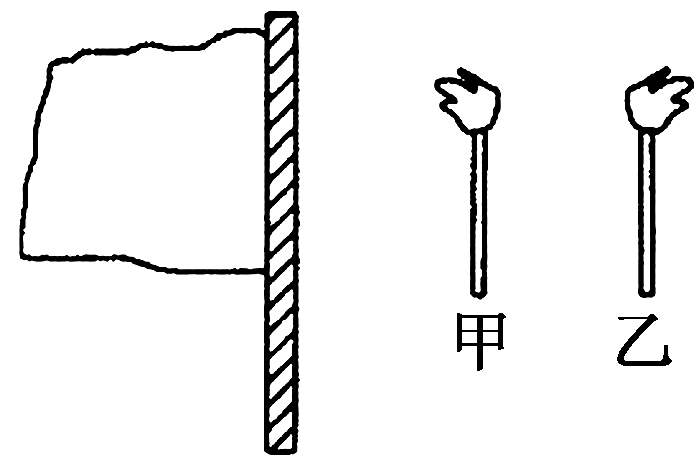
\includegraphics{../picture/1-1/001.png}
   中的旗帜和甲、乙两火炬手所传递的圣火火焰。关于甲、乙两火炬手相对于静止旗杆的运动情况,下列说法中正确的是(旗杆和甲、乙两火炬手在同一地区)
   \choice[A]甲、乙两火炬手一定向左运动
   \choice[B]甲、乙两火炬手一定向右运动
   \choice[C]甲火炬手可能运动,乙火炬手向右运动
   \choice[D]甲火炬手可能静止,乙火炬手向左运动
\end{xuanze}

\subsubsection{位移和路程}

\begin{xuanze}
   4.关于位移和路程,下列说法正确的是()
   \choice[A]在某一段时间内物体运动的位移为零,则该物体一定是静止的
   \choice[B]在某一段时间内物体运动的路程为零,则该物体一定是静止的
   \choice[C]在直线运动中,物体的位移大小一定等于其路程
   \choice[D]在曲线运动中,物体的位移大小可能等于路程

   5.(多选)在机器人大赛中,某机器人在平面内由点(0,0)出发,沿直线运动到点(3,1),然后又由点(3,1)沿直线运动到点(1,4),然后又由点(1,4)沿直线运动到点(5,5),最后又由点(5,5)沿直线运动到点(2,2),平面坐标系横、纵坐标轴的单位长度为 1 m。整个过程中机器人所用时间是 $2\sqrt{2}s$, 则
   \choice[A]机器人的运动轨迹是一条直线
   \choice[B]机器人不会两次通过同一点
   \choice[C]整个过程中机器人的位移大小为 $2\sqrt{2} m$
   \choice[D]整个过程中机器人的位移与由点(5,5)运动到点(2,2)的位移方向相反

\end{xuanze}

\subsubsection{平均速度和瞬时速度}

\begin{xuanze}
   6.如
   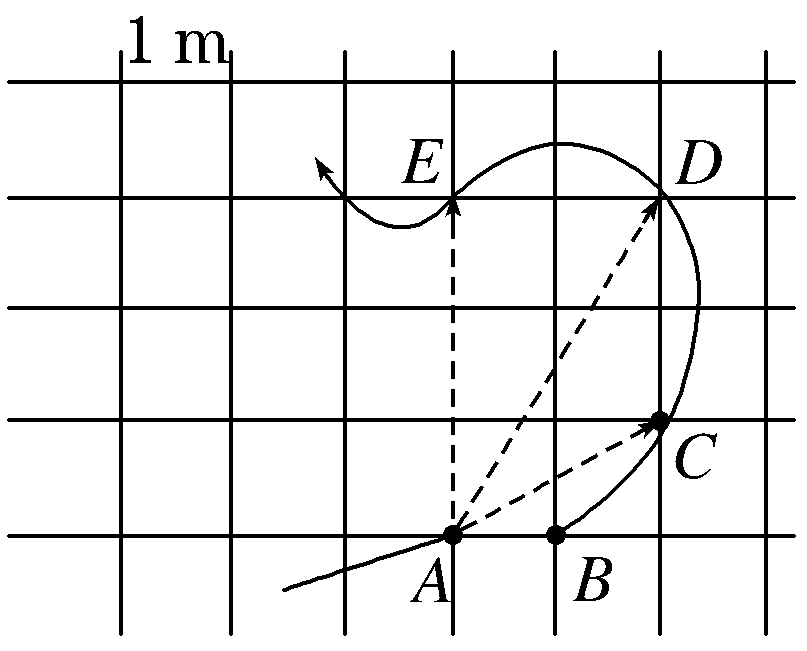
\includegraphics{../picture/1-1/002.png}
   所示,物体沿曲线轨迹的箭头方向运动,AB、ABC、ABCD、ABCDE 四段曲线轨迹运动所用的时间分别是:1 s、2 s、3 s、4 s。下列说法不正确的是
   \choice[A]物体在 AB 段的平均速度为 $1 m/s$
   \choice[B]物体在 ABC 段的平均速度为$ \tfrac{\sqrt{5}}{2} m/s$
   \choice[C]AB 段的平均速度比 ABC 段的平均速度更能反映物体处于 A 点时的瞬时速度
   \choice[D]物体在 B 点的速度等于 AC 段的平均速度

   7.一质点沿直线 Ox 方向做变速运动,它离开 O 点的距离 x 随时间 t 变化的关系为 $x=(5+2t^3)m$,它的速度随时间 t 变化的关系为 $v=6t^2m/s$,该质点在 $t=0$ 到 $t=2 s$ 间的平均速度和 $t=2 s$ 到 $t=3 s$ 间的平均速度的大小分别为
   \choice[A] $12 m/s$\quad $39 m/s$
   \choice[B] $8 m/s$\quad $38 m/s$
   \choice[C] $12 m/s$\quad  $19.5 m/s$
   \choice[D] $8 m/s$\quad $13 m/s$

\end{xuanze}

\begin{jisuan}
   8.为了测定气垫导轨上滑块的加速度,滑块上安装了宽度为 3.0 cm 的遮光板,如
   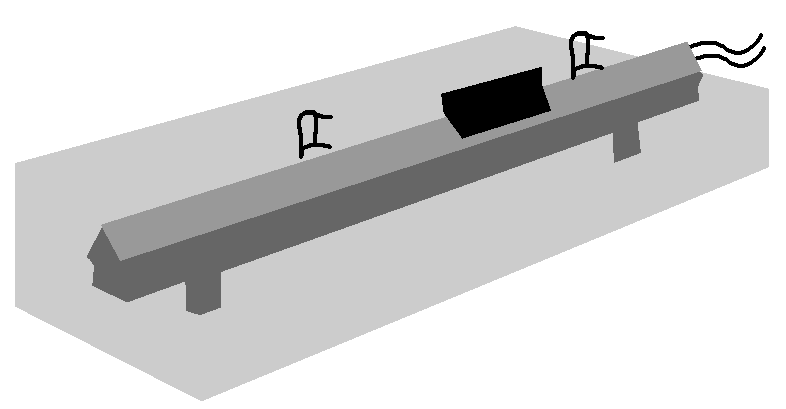
\includegraphics{../picture/1-1/003.png}
所示,滑块在牵引力作用下先后匀加速通过两个光电门,配套的数字毫秒计记录了遮光板通过第一个光电门的时间为$\Delta t_1=0.30 s$,通过第二个光电门的时间为 $\Delta t_2=0.10 s$,遮光板从开始遮住第一个光电门到开始遮住第二个光电门的时间为 $\Delta t=3.0 s$。试估算:
\qitem 滑块的加速度多大(保留两位有效数字)?
\qitem 两个光电门之间的距离是多少?

\end{jisuan}

\subsubsection{速度和加速度}
\begin{xuanze}
   9.下面关于加速度的描述中正确的有
\choice[A]加速度描述了物体速度变化的多少
\choice[B]加速度在数值上等于单位时间里速度的变化量
\choice[C]当加速度与位移方向相反时,物体做减速运动
\choice[D]当加速度与速度方向相同且又减小时,物体做减速运动

10.关于速度、速度的变化和加速度的关系,下列说法中正确的是
\choice[A]速度变化的方向为正,加速度的方向为负
\choice[B]物体加速度增大,速度一定越来越大
\choice[C]速度越来越大,加速度一定越来越大
\choice[D]加速度可能既不与速度同向,也不与速度反向

11.一个质点做速度方向不变的直线运动,加速度的方向始终与速度方向相同,但加速度大小逐渐减小直至为零,在此过程中
\choice[A]速度逐渐减小,当加速度减小到零时,速度达到最小值
\choice[B]速度逐渐增大,当加速度减小到零时,速度达到最大值
\choice[C]位移逐渐增大,当加速度减小到零时,位移将不再增大
\choice[D]位移逐渐减小,当加速度减小到零时,位移达到最小值

12.关于重力加速度,下列说法正确的是
\choice[A]在比萨斜塔上同时由静止释放一大一小两个金属球,两球同时着地,说明两球运动
\choice[B] 速度相同,这个加速度就是当地的重力加速度
\choice[C]地球上各处的重力加速度 g 的值都相同
\choice[D]济南的重力加速度为 $9.8 m/s^2$,说明在济南做下落运动的物体,每经过 $1 s$ 速度增加$9.8 m/s$ 哈尔滨和广州的重力加速度都竖直向下,两者的方向相同

\end{xuanze}


\section{匀变速直线运动的规律}
\subsection{匀变速直线运动的基本规律}
\begin{xuanze}
   1.以 $36 km/h$ 的速度沿平直公路行驶的汽车,遇障碍物刹车后获得大小为 $a=4 m/s^2$ 的加速度,刹车后\CJKunderwave{第 $3 s$ 内},汽车走过的路程为 
  \choice[A] $12.5 m$
  \choice[B] $2m$
  \choice[C] $10m$
  \choice[D] $0.5$

  2.在\CJKunderwave{光滑足够长}的斜面上,有一物体以 $10 m/s$ 初速度沿斜面向上运动,如果物体的加速度始终为 $5 m/s^2$,方向沿斜面向下。那么经过 $3 s$ 时的速度大小和方向是
\choice[A] $25 m/s$,沿斜面向上
\choice[B] $5 m/s$,沿斜面向下
\choice[C] $5 m/s$,沿斜面向上
\choice[D] $25 m/s$,沿斜面向下

\end{xuanze}

\subsection{解决匀变速直线运动的常用方法}

\begin{xuanze}
  3.做匀减速直线运动的物体经 $4s$ 后停止,若在第 $1s$ 内的位移是 $14m$,则最后 $1s$ 的位移是
\choice[A] $3.5m$
\choice[B] $2m$
\choice[C] $1m$
\choice[D] $0$
   
4.一物体做匀加速直线运动,通过一段位移 $\Delta x$ 所用的时间为 $t_1$,紧接着通过下一段位移 $\Delta x$ 所用的时间为 $t_2$。则物体运动的加速度为
\choice[A] $\cfrac{2\Delta x(t_1-t_2)}{t_1t_2(t_1+t_2)}$
\choice[B] $\cfrac{\Delta x(t_1-t_2)}{t_1t_2(t_1+t_2)}$
\choice[C] $\cfrac{2\Delta x(t_1+t_2)}{t_1t_2(t_1-t_2)}$
\choice[D] $\cfrac{\Delta x(t_1+t_2)}{t_1t_2(t_1-t_2)}$

\end{xuanze}

\subsection{自由落体和竖直上抛运动}

\begin{jisuan}
5.如
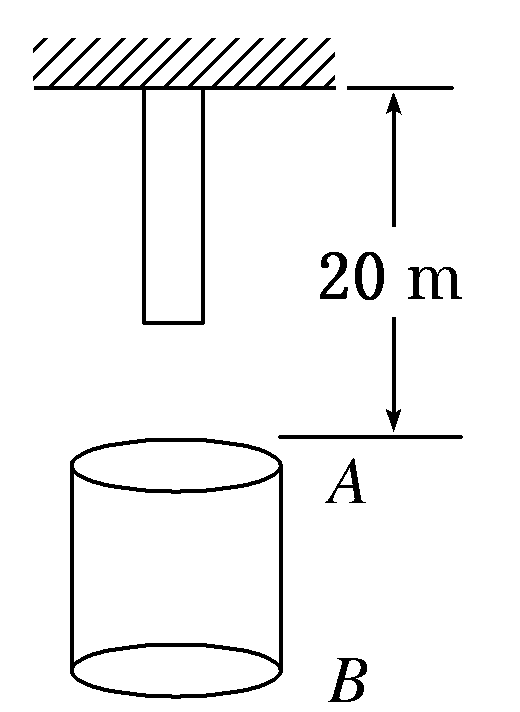
\includegraphics{../picture/1-2/001.png}
所示木杆长 $5m$,上端固定在某一点,由静止放开后让它自由落下(不计空气阻力),木杆通过悬点正下方 $20m$ 处圆筒 AB,圆筒 AB 长为 $5m$,求:
\qitem 木杆经过圆筒的上端A所用的时间$t_1$是多少?
\qitem 木杆通过圆筒AB所用的时间$t_2$是多少?(取 $g=10 m/s^2$)

\end{jisuan}

\begin{xuanze}
6.在离地高$h$处,沿竖直方向同时向上和向下抛出两个小球,它们的初速度大小均为$v$,不计空气阻力,两球落地的时间差为
\choice[A] $\cfrac{2v}{g}$
\choice[B] $\cfrac{v}{g}$
\choice[C] $\cfrac{2h}{v}$
\choice[D] $\cfrac{h}{v}$
   
\end{xuanze}

\subsection{利用思维转换法巧解匀变速直线运动问题}

\begin{xuanze}
8.一物块(可看成质点)以一定的初速度从一光滑斜面底端 A 点上滑,最高可滑到 C 点,已知 AB 是 BC 的 3 倍,如
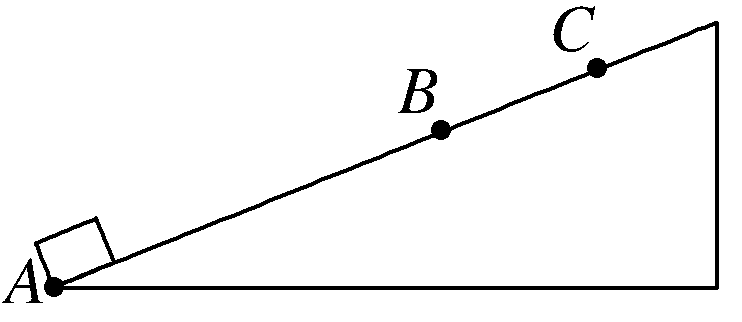
\includegraphics{../picture/1-2/002.png}
所示,已知物块从 A 至 B 所需时间为 $t_0$,则它从 B 经 C 再回到 B,需要的时间是
\choice[A] $t_0$
\choice[B] $\cfrac{t_0}{4}$
\choice[C] $2t_0$
\choice[D] $\cfrac{t_0}{2}$

9.如
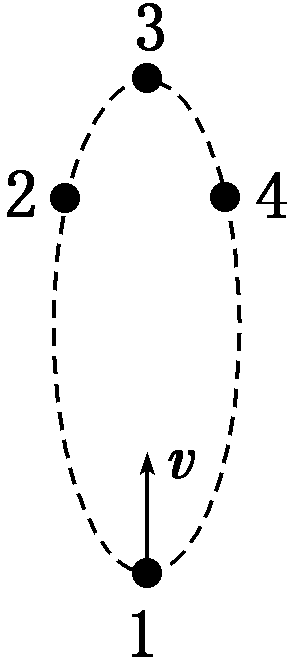
\includegraphics{../picture/1-2/003.png}
所示,一杂技演员用一只手抛球、接球,他每隔 $0.4s$ 抛出一球,接到球便立即把球抛出。已知除抛、接球的时刻外,空中总有 4 个球,将球的运动近似看做是竖直方向的运动,球到达的最大高度是(高度从抛球点算起,取 $g=10 m/s^2$)
\choice[A] $1.6m$
\choice[B] $2.4m$
\choice[C] $3.2m$
\choice[D] $4.0m$

10.如
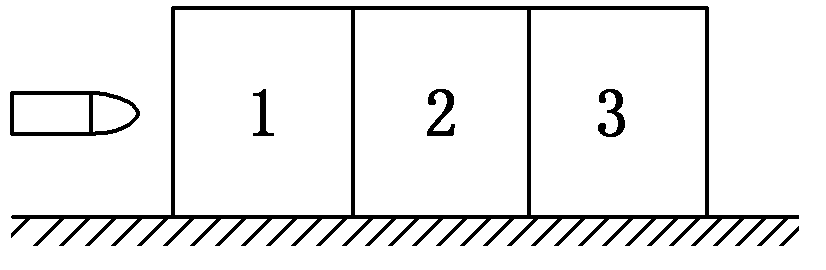
\includegraphics{../picture/1-2/004.png}
所示,在水平面上固定着三个完全相同的木块,一子弹以水平速度射入木块,若子弹在木块中做匀减速直线运动,当穿透第三个木块时速度恰好为零,则子弹依次射入每个木块时的速度比和穿过每个木块所用时间比分别为
\choice[A] $v_1:v_2:v_3=3:2:1$
\choice[B] $v_1:v_2:v_3=\sqrt{5}:\sqrt{3}:1$
\choice[C] $\Delta t_1:\Delta t_2:\Delta t_3 =1:\sqrt{2}:\sqrt{3}$
\choice[D] $\Delta t_1:\Delta t_2:\Delta t_3 =\sqrt{3}-\sqrt{2}:\sqrt{2}-1:1$

\end{xuanze}

\begin{jisuan}
11.从斜面上某一位置每隔 0.1 s 释放一颗小球,在连续释放几颗后,对斜面上正在运动着的小球拍下部分照片,如
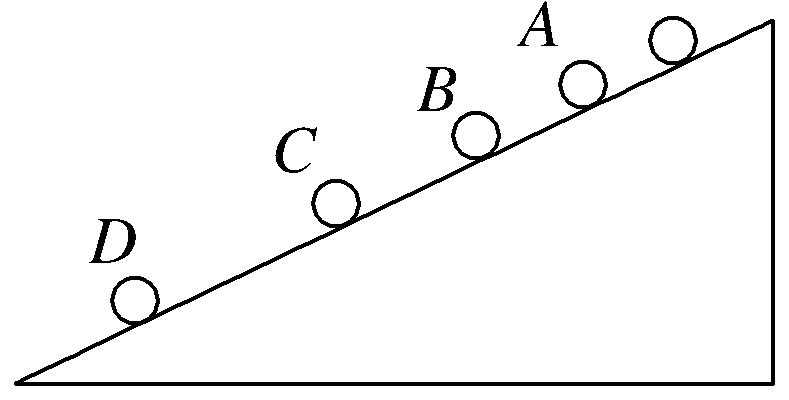
\includegraphics{../picture/1-2/005.png}
所示。现测得 $x_{AB}=15 cm$,$x_{BC}=20 cm$,已知小球在斜面上做匀加速直线运动,且加速度大小相同。
\qitem 求小球的加速度
\qitem 求拍摄时B球的速度
\qitem D、C两球相距多远?
\qitem A球上面正在运动着的小球共有几颗?

\end{jisuan}

\section{运动图象、追击与相遇问题}

\subsection{三类运动图像的比较}
\begin{xuanze}
   1.如
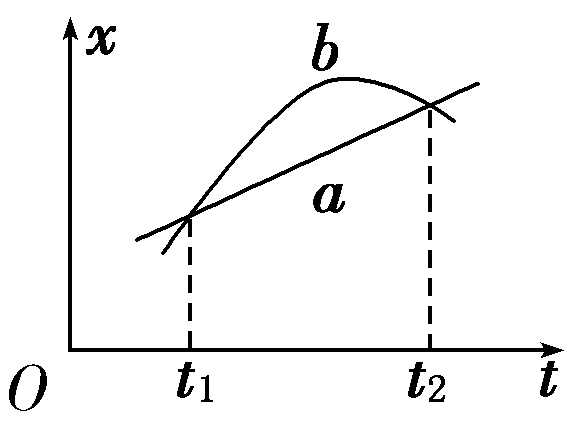
\includegraphics{../picture/1-3/001.png} 
所示直线 a 和曲线 b 分别是在平直公路上行驶的汽车 a 和 b 的位置-时间($x-t$)图线。由图可知
\choice[A] 在时刻$t_1$,a 车追上 b 车
\choice[B] 在时刻$t_2$,a、b 两车运动方向相反
\choice[C] 在$t_1$到$t_2$这段时间内,b 车的位移比 a 车的大
\choice[D] 在$t_1$到$t_2$这段时间内,b 车的速率一直比 a 车的大

2.(多选)
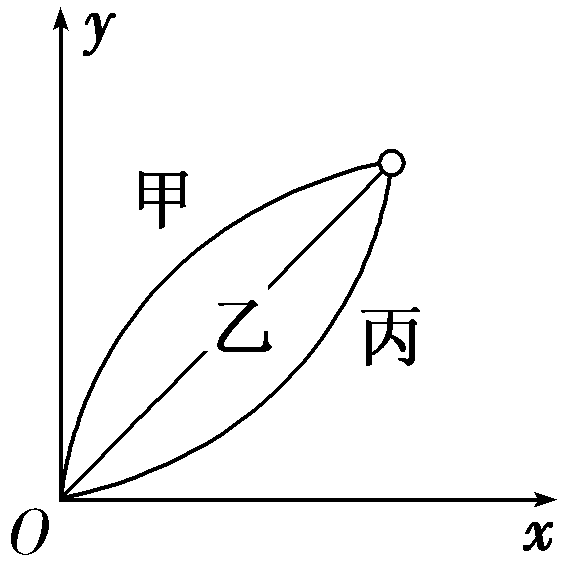
\includegraphics{../picture/1-3/002.png} 
为甲、乙、丙三个军事小分队进行军事行动的运动图像,下列说法正确的是
\choice[A] 甲、丙两个分队的运动路线为曲线,乙分队的运动路线为直线
\choice[B] 甲、乙、丙三个分队的位移相等
\choice[C] 甲、乙、丙三个分队的平均速度相等
\choice[D] 甲、乙、丙三个分队运动的路程相等

3.甲、乙两汽车在一平直公路上同向行驶。在 $t=0$ 到 $t=t_1$ 的时间内,它们的 $v-t$ 图像如
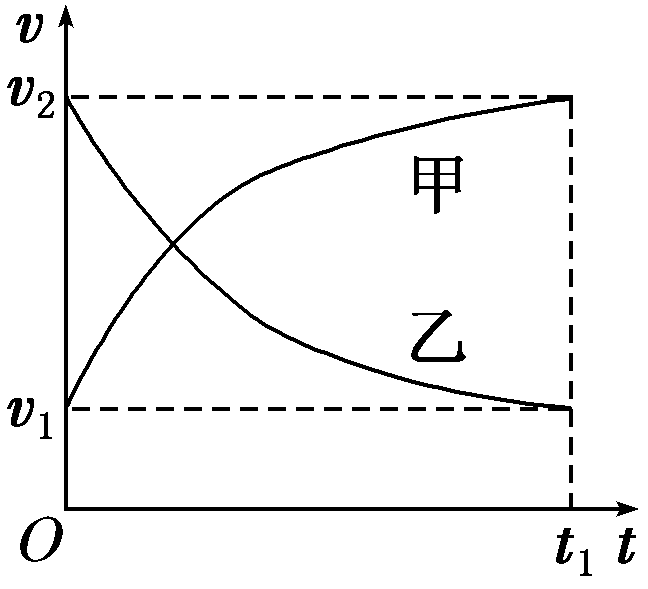
\includegraphics{../picture/1-3/003.png} 
所示。在这段时间内
\choice[A] 汽车甲的平均速度比乙的大
\choice[B] 汽车乙的平均速度等于$\cfrac{v_1+v_2}{2}$
\choice[C] 甲、乙两汽车的位移相同
\choice[D] 汽车甲的加速度大小逐渐减小,汽车乙的加速度大小逐渐增大

\end{xuanze}

\subsection{图像问题的解题思路}

\begin{jisuan}
   4.一汽车从静止开始做匀加速直线运动,然后刹车做匀减速直线运动,直到停止。下列速度 v 和位移 x 的关系
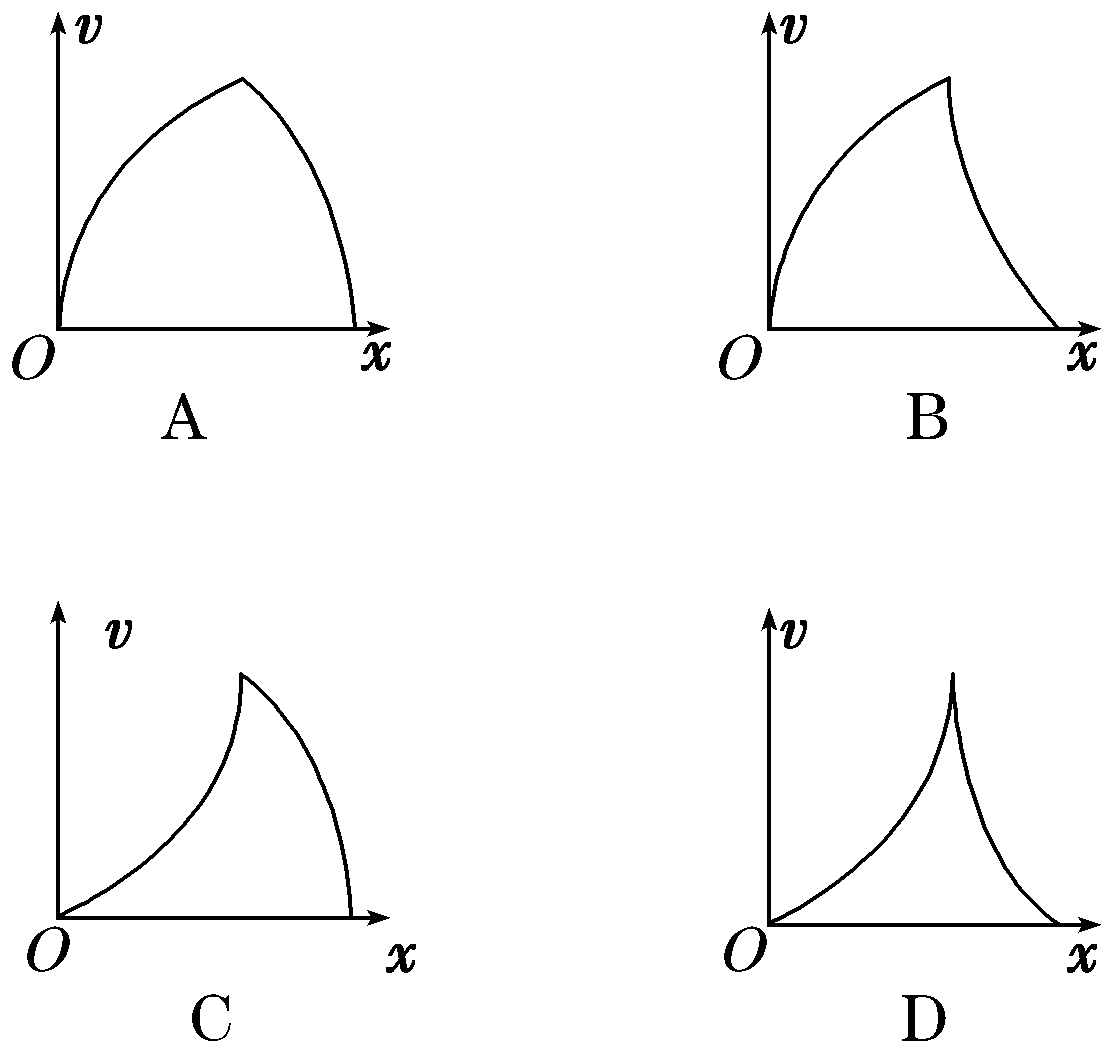
\includegraphics{../picture/1-3/004.png} 
中,能描述该过程的是

   5.一物体由静止开始沿直线运动,其加速度随时间变化的规律如
   <BeginPicture>
   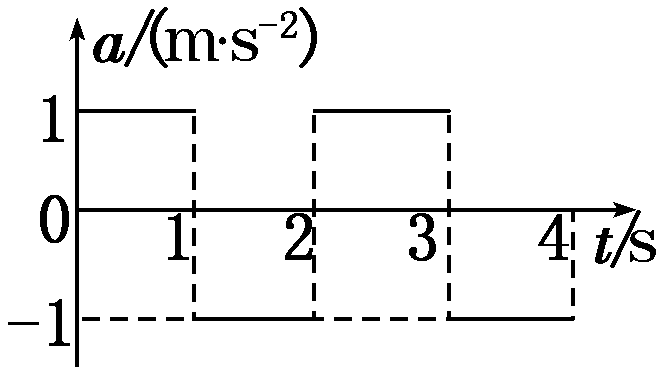
\includegraphics{../picture/1-3/005.png} 
   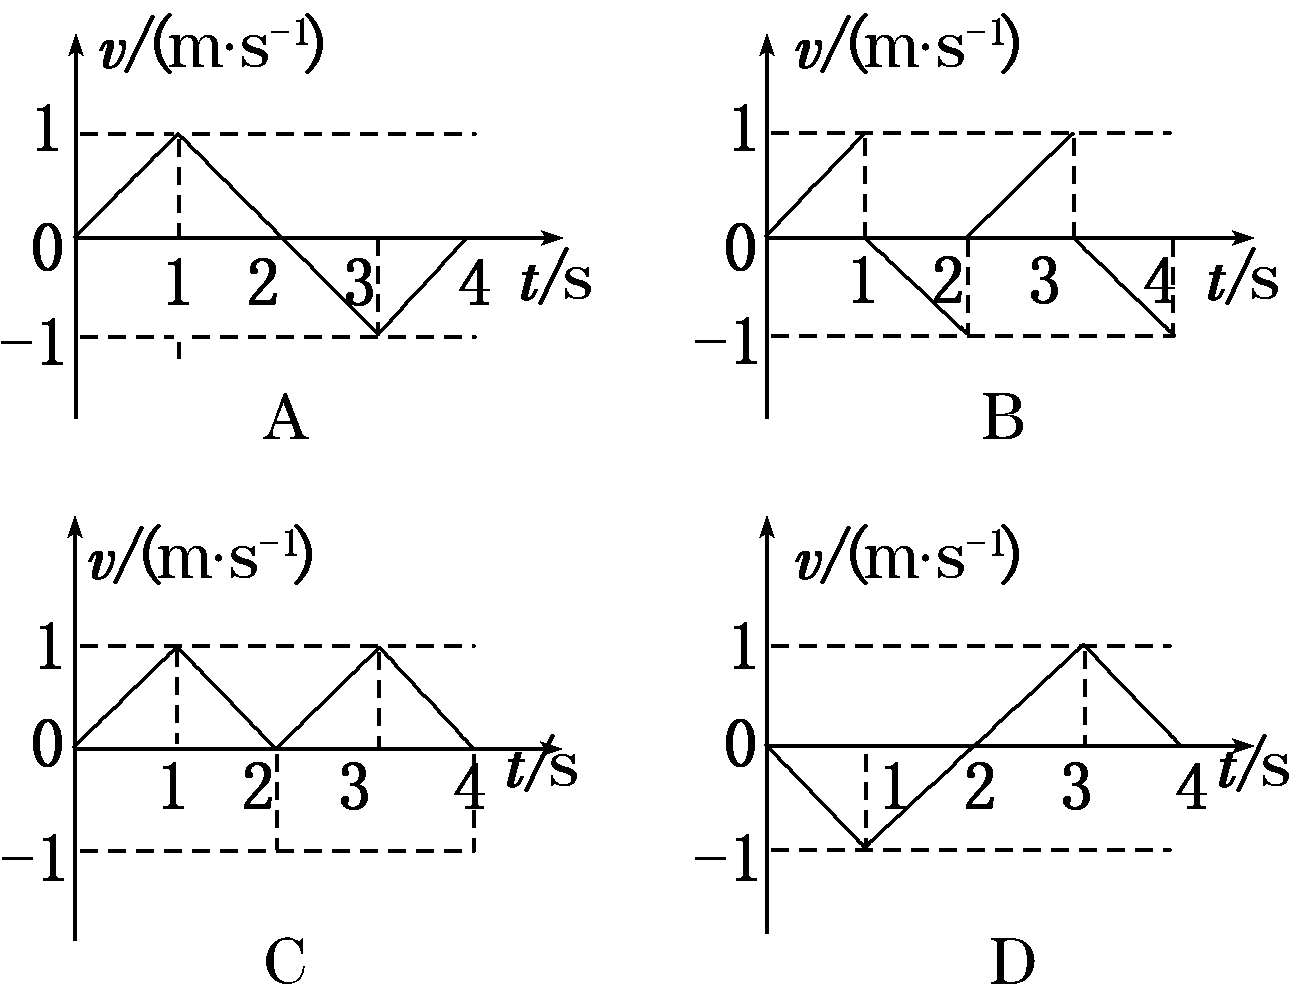
\includegraphics{../picture/1-3/006.png} 
   <EndPicture>
   所示。取物体开始运动的方向为正方向,则下列关于物体运动的$v-t$图像正确的是

\end{jisuan}

\begin{xuanze}
6.某同学以校门口为原点,向东方向为正方向建立坐标,记录了甲、乙两位同学的位移—时间($x-t$)图线,如
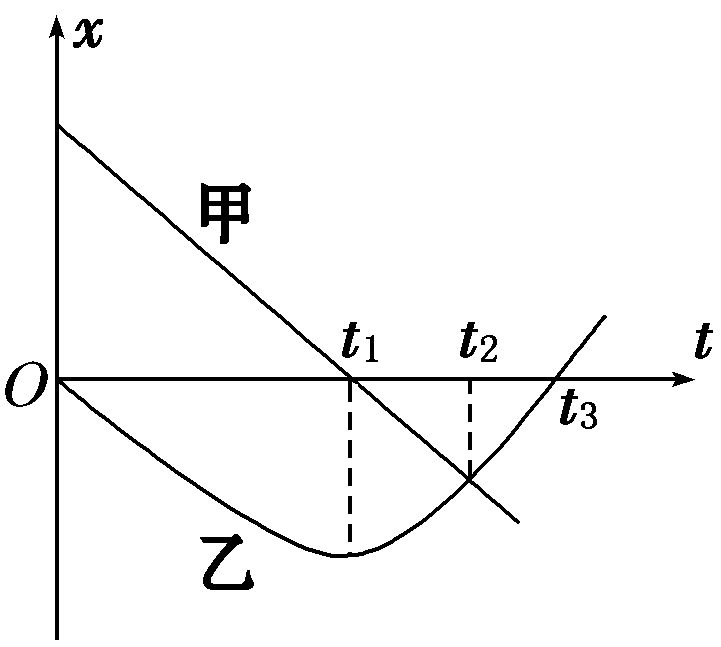
\includegraphics{../picture/1-3/007.png} 
所示,下列说法中正确的是
\choice[A] 在 $t_1$ 时刻,甲的瞬时速度为零,乙的速度不为零
\choice[B] 在 $t_2$ 时刻,甲、乙速度可能相同
\choice[C] 在 $t_2$ 时刻,甲、乙两同学相遇
\choice[D] 在 $t_3$ 时刻,乙的速度为零、加速度不为零

\end{xuanze}





\end{document}
